\documentclass[10pt,aspectratio=169]{beamer}

% All the boilerplate is in deslides.sty
\usepackage{deslides}

\author{Ji\v{r}\'i Lebl}

\institute[OSU]{%
Oklahoma State University%
%Departemento pri Matematiko de Oklahoma {\^S}tata Universitato%
}

\title{5. Separable equations (Notes on Diffy Qs, 1.3)}

\date{}

\begin{document}

\begin{frame}
\titlepage

%\bigskip

\begin{center}
The textbook: \url{https://www.jirka.org/diffyqs/}
\end{center}
\end{frame}

\begin{frame}
Given
$y' = f(x)$ we integrate to solve: $y = \int f(x) \,dx + C$. 

\medskip
\pause

Similarly we could solve $y' = f(y)$ by writing $x$ in terms of $y$.

\medskip
\pause

But the strategy doesn't work for the general $y' = f(x,y)$.

\medskip
\pause

Integrating yields
\[
y = \int f(x,y) \,dx + C .
\]

\medskip
\pause

But if the equation is so called ``separable,'' then we can
still integrate.

\end{frame}

\begin{frame}

A differential equation is \emph{separable} if we can write it as
\[
y' = f(x)g(y) ,
\]
\pause
Using the Leibniz notation $\frac{dy}{dx} = f(x)g(y)$, rewrite it as
\[
\frac{dy}{g(y)} = f(x) \,dx .
\]
\pause
Now we could integrate both sides:
\[
\int \frac{dy}{g(y)} = \int f(x) \,dx + C .
\]
\pause
We now solve for $y$ (if you can).

\end{frame}

\begin{frame}

\textbf{Example:}
Consider
$y' = xy$.

\medskip
\pause

$y=0$ is a solution, so remember that and assume $y\not= 0$ from now.

\medskip
\pause

Write: \qquad $\displaystyle \frac{dy}{dx} = xy$
\pause
\qquad Integrate:
$\displaystyle
\int \frac{dy}{y} = \int x\,dx + C$
\pause
\wthus
$\displaystyle
\ln \, \lvert y\rvert = \frac{x^2}{2} + C$

\medskip
\pause

\thus\quad
$\displaystyle \lvert y \rvert = e^{\frac{x^2}{2} + C}
\pause
 = e^C e^{\frac{x^2}{2}}$

\medskip
\pause

$e^C$ is an arbitrary positive constant.

\pause
Because of the absolute value we could replace it with a negative.

\pause
And $y=0$ is also a solution.

\medskip
\pause

So the general solution is \quad $\displaystyle y = D e^{\frac{x^2}{2}}$
\quad ($D$ a constant).

\medskip
\pause

Check:
$\displaystyle
y' \pause = D x e^{\frac{x^2}{2}} \pause = x \left( D e^{\frac{x^2}{2}}
\right) \pause = xy$.
\qquad
{\Large\checkmark}
\end{frame}

\begin{frame}
It appears as if we are integrating with two different variables.

\medskip
\pause

So why does it work?

\medskip
\pause

Note that $y=y(x)$ and $\dfrac{dy}{dx}$ are functions of $x$.

\medskip
\pause

Write
\quad
$\displaystyle \frac{dy}{dx} = f(x)g(y)$
\quad
as
\quad
$\displaystyle
\frac{1}{g(y)}\,\frac{dy}{dx} = f(x)$.

\medskip
\pause

Now integrate both sides wrt $x$:
\quad
$\displaystyle
\int \frac{1}{g(y)}\,\frac{dy}{dx} \,dx = \int f(x) \,dx + C$.

\medskip
\pause

Substitution formula from calculus says
\quad $\displaystyle
\int \frac{1}{g(y)}\,dy = \int f(x) \,dx + C$.
\quad
{\Large\checkmark}

\end{frame}

%FIXME: not done from here

\begin{frame}
We sometimes get stuck even if we can do the
integration.  Consider the separable equation
\begin{equation*}
y' = \frac{xy}{y^2+1} .
\end{equation*}
We separate variables,
\begin{equation*}
\frac{y^2+1}{y}\,dy = \left(y+\frac{1}{y}\right)\,dy = x\,dx .
\end{equation*}
We integrate to get
\begin{equation*}
\frac{y^2}{2} + \ln \, \lvert y \rvert = \frac{x^2}{2} + C ,
\end{equation*}
or perhaps the easier looking expression (where $D = 2C$)
\begin{equation*}
y^2 + 2 \ln \, \lvert y\rvert = x^2 + D .
\end{equation*}
It is not easy to find the solution explicitly as it is hard to solve
for $y$.  We, therefore, leave the solution in this form and call
it an
\emph{implicit solution}.
It is still
easy to check that an implicit solution satisfies the differential
equation.  In this case, we differentiate with respect to $x$, and remember
that $y$ is a function of $x$,
to get
\begin{equation*}
y'\left(2y + \frac{2}{y}\right) = 2x .
\end{equation*}
Multiply both sides by $y$ and divide by $2(y^2+1)$ and you will
get exactly the differential equation.  We leave this computation to the
reader.

If you have an implicit solution, and
you want to compute values
for $y$, you might have to be tricky.  You might get multiple solutions $y$
for each $x$, so you have to pick one.  Sometimes you can
graph $x$ as a function of $y$, and then flip your paper.
Sometimes you have to do more.

Computers are also good at some of these tricks.
More advanced mathematical software usually has some
way of plotting solutions to implicit equations.
For example, for $C=0$ if you plot all the points $(x,y)$ that
are solutions to $y^2+2\ln|y|=x^2$,
you find the two curves in {implicitsols:fig}.  This is not quite
a graph of a function. For each $x$ there are two choices of $y$.
To find a function you would have to pick one of these two curves.
You pick the one that satisfies your initial condition if you have one.
For example, the top curve satisfies the condition $y(1)=1$.
So for each $C$ we really got two solutions.
As you can see, computing values from an implicit solution can be somewhat
tricky.  But sometimes, an implicit solution is the best we can do.

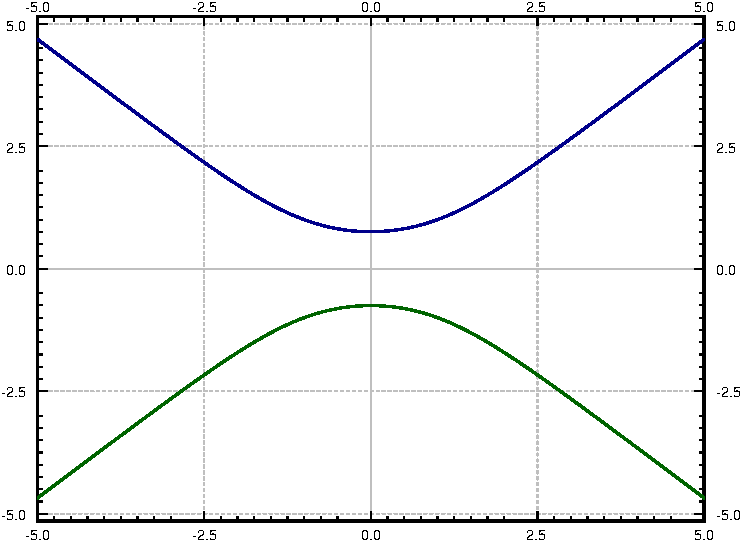
\includegraphics[width=3in]{../figures/implicitsols}

The implicit solution $y^2+2\ln|y|=x^2$ to $y'=\frac{xy}{y^2+1}$.


The equation above also has the solution $y=0$.
So the general solution is 
\begin{equation*}
y^2 + 2 \ln \, \lvert y \rvert = x^2 + C, \qquad \text{and} \qquad y=0.
\end{equation*}
These outlying solutions
such as $y=0$
are sometimes called \emph{singular solutions}.

{Examples of separable equations}

\begin{example}
Solve $x^2y' = 1 - x^2+y^2 - x^2y^2$, $y(1) = 0$.

Factor the right-hand side
\begin{equation*}
x^2y' = (1 - x^2)(1+y^2) .
\end{equation*}
Separate variables, integrate, and solve for $y$:
\begin{align*}
\frac{y'}{1+y^2} & = \frac{1 - x^2}{x^2} , \\
\frac{y'}{1+y^2} & = \frac{1}{x^2} - 1 , \\
\operatorname{arctan} (y) & = \frac{-1}{x} - x + C , \\
y & = \tan \left(\frac{-1}{x} - x + C\right) .
\end{align*}
Solve for the initial condition, $0 = \tan(-2+C)$ to get $C=2$ (or $C = 2 +
\pi$, or $C = 2 + 2\pi$, etc.).  The particular solution we seek is, therefore,
\begin{equation*}
y = \tan \left(\frac{-1}{x} - x + 2 \right) .
\end{equation*}
\end{example}

\textbf{Example:}
Bob made a cup of coffee, and
Bob likes to drink coffee only once reaches 60 degrees Celsius and will not burn him.
Initially at time $t=0$ minutes,
Bob measured the temperature and the coffee was 89 degrees Celsius.
One minute later, Bob measured the coffee again and it had 85 degrees.
The temperature of the room (the ambient temperature) is 22 degrees.
When should Bob start drinking?

Let $T$ be the temperature of the coffee in degrees Celsius, and let $A$ be
the ambient (room) temperature, also in degrees Celsius.
Newton's law of cooling states that the rate at which the
temperature of the coffee is changing
is proportional to the difference between the
ambient temperature and the temperature of the coffee.  That is,
\begin{equation*}
\frac{dT}{dt} = k(A-T) ,
\end{equation*}
for some constant $k$.
For our setup $A=22$, $T(0) = 89$, $T(1) = 85$.
We separate variables and integrate (let $C$ and $D$ denote arbitrary
constants):
\begin{align*}
\frac{1}{T-A} \, \frac{dT}{dt} & = -k , \\
\ln (T-A) &= -kt + C , \qquad \text{(note that } T-A > 0 \text{)} \\
T-A &= D\, e^{-kt} ,  \\
T &= A + D\, e^{-kt} .
\end{align*}
That is,
$T = 22 + D\, e^{-kt}$.  We plug in the first condition: $89 = T(0) = 22 +
D$,
and hence $D = 67$.  So
$T = 22 + 67\, e^{-kt}$.  The second condition says $85 = T(1) = 
22 + 67\, e^{-k}$.  Solving for $k$ we get
$k = - \ln \frac{85-22}{67} \approx 0.0616$.  Now we solve for the time $t$
that gives us a temperature of 60 degrees.  Namely, we solve
\begin{equation*}
60 = 22 + 67 e^{-0.0616t}
\end{equation*}
to get
$t = - \frac{\ln \frac{60-22}{67}}{0.0616} \approx 9.21$ minutes.  So Bob can
begin to drink the coffee at just over 9 minutes from the time Bob made
it.  That is probably about the amount of time it took us to calculate how long
it would take.  See {sintro:coffeefig}.

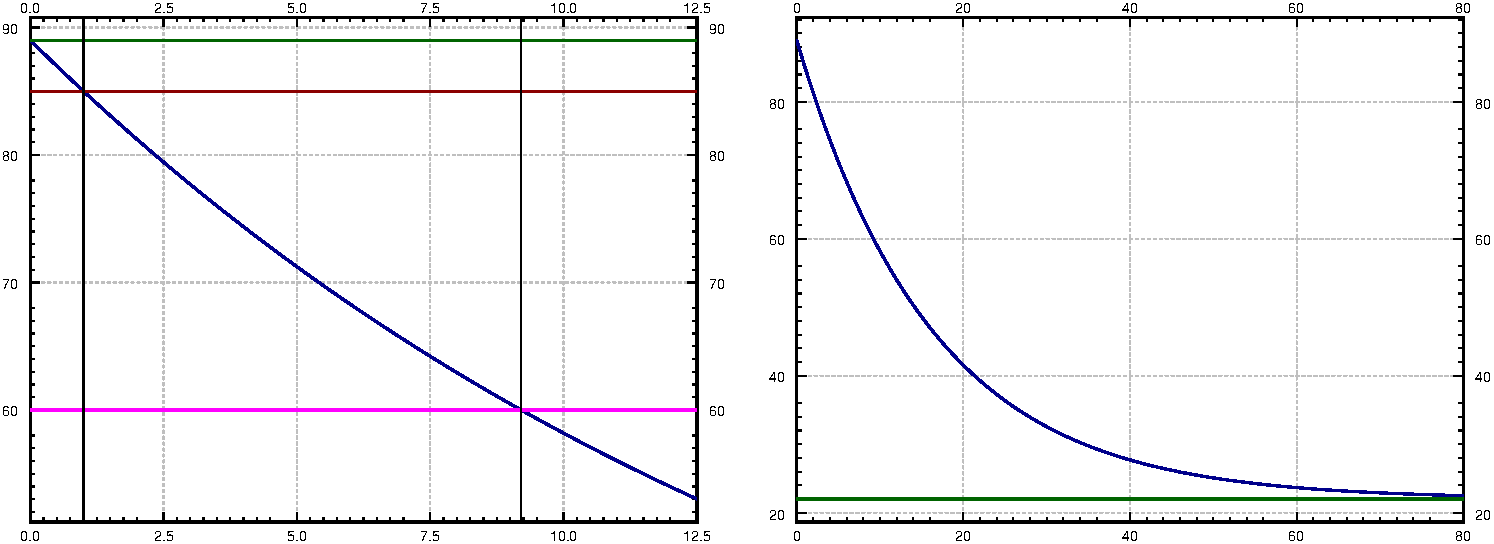
\includegraphics[width=6.24in]{../figures/coffeefig-1-2}

Graphs of the coffee temperature function $T(t)$.
On the left, horizontal
lines are drawn at temperatures 60, 85, and 89.  Vertical lines
are drawn at $t=1$ and $t=9.21$.  Notice that the
temperature of the coffee hits 85 at $t=1$, and 60 at
$t \approx 9.21$.  On the right, the graph is over a longer period of time,
with a horizontal line at the ambient temperature 22.

\end{frame}

\begin{frame}

\textbf{Example:}
Find the general solution to $y' = \frac{-xy^2}{3}$ (including singular
solutions).

First note that $y=0$ is a solution (a singular solution).
Now assume that $y \not= 0$.
\begin{align*}
\frac{-3}{y^2} y' & = x , \displaybreak[0]\\
\frac{3}{y} & = \frac{x^2}{2} + C , \displaybreak[0]\\
y & = \frac{3}{\nicefrac{x^2}{2} + C}
= \frac{6}{x^2 + 2C}.
\end{align*}
So the general solution is,
\begin{align*}
y = \frac{6}{x^2 + 2C}, \qquad \text{and} \qquad y=0 .
\end{align*}

\end{frame}

\end{document}
